\section{JavaScript and JavaScript Frameworks}
\label{litrev:javascript}
JavaScript has existed for many years and is now one of the most widely known and used front-end programming languages in web development (\cite{mariano_benchmarking_nodate}). Due to the language's wide popularity within web development, various frameworks have been developed to extend the pre-existing functionality of vanilla JavaScript. JavaScript frameworks enable web development by utilising a component-based approach, allowing for these components to be designed and developed to be reused. Creating reusable components aids in reducing the software development time and increasing the reliability of the product (\cite{crnkovic_challenges_2002}).

There are a range of different JavaScript frameworks that both increase and decrease in popularity over time. React, Vue and Angular are at the current forefront of JavaScript frameworks, whereas other frameworks, such as JQuery, used to be popular but have recently decreased in popularity. The Stack Overflow insights tool demonstrates the decline in user questions surrounding different JavaScript frameworks, paralleling the decline of JQuery and the adoption of React, Vue, and Angular \see{fig:so-trends}.

\begin{figure}
    \centering
    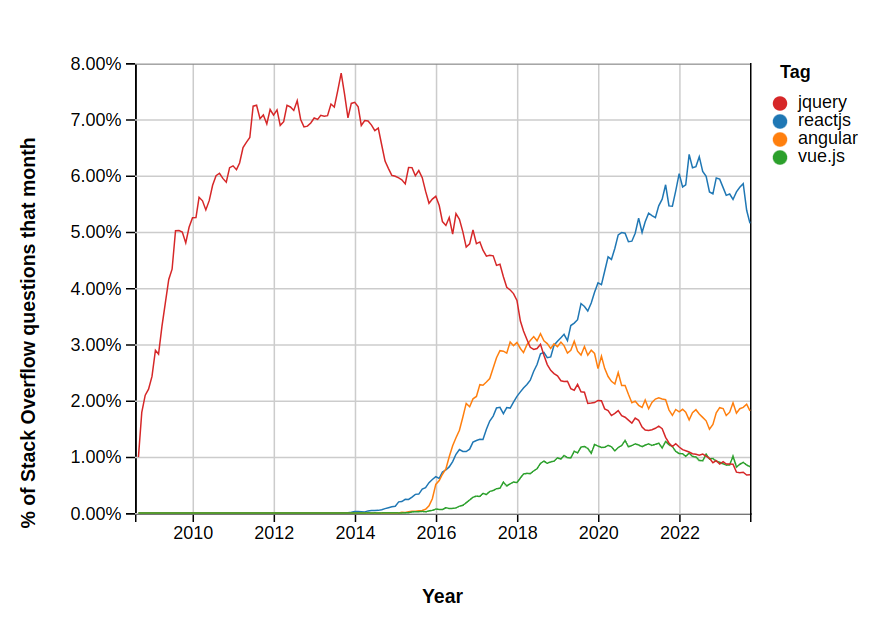
\includegraphics[width=0.9\linewidth]{figures/so-trends.png}
    \caption{Stack Overflow Trends JavaScript Frameworks (14/11/2023) (\cite{noauthor_stack_nodate})}
    \label{fig:so-trends}
\end{figure}

\begin{figure}
    \centering
    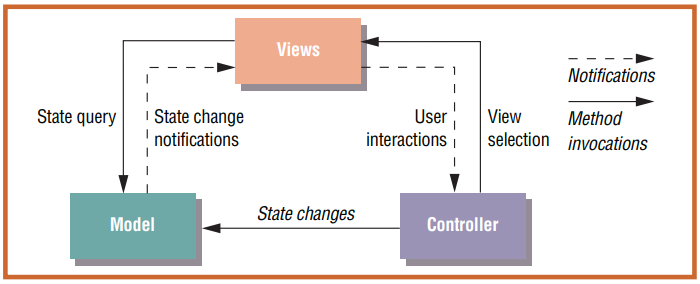
\includegraphics[width=0.9\linewidth]{figures/MVC.png}
    \caption{Model View Controller Model (\cite{curry_flexible_2008})}
    \label{fig:mvc-model}
\end{figure}

\clearpage

\subsection{React} 
\label{litrev:react}

The React.js framework was originally built by software engineers at Facebook with the intention of developing a JavaScript library for building user interfaces. React's main focus is to enable developers to "combine a number of short independent code fragments into a complex UI interface" (\cite{xu_benchmark_nodate}). React works similarly to the MVC (Model View Controller) model \see{fig:mvc-model}; it simply acts as the 'View' part of the model where it interacts with and utilises the VDOM (Virtual Document Object Model). When a state or props change occurs for a component, React compares the newly returned VDOM component with the previously rendered DOM component. If these components are not equal, the entire DOM is re-rendered (\cite{mariano_benchmarking_nodate}). 

\subsection{Next.js}
\label{litrev:next}

Next.js is a framework built on the original React.js framework and has recently become the new default for new React projects. It natively incorporates multiple production-ready such as server-side rendering. This feature, in particular, is one key improvement Next.js introduces whereby JavaScript modules are dynamically loaded on the server, drastically decreasing the client-side loading times (\cite{dinku_reactjs_2022}). Despite these improvements to React, introducing features such as server-side rendering can reduce the framework's compatibility with libraries such as Leaflet for OpenStreetMap which is pivotal to this project.

\subsection{Vue}
\label{litrev:vue}

In contrast to React, Vue was released in 2014, and instead of being built from the MVC model, it uniquely provides MVVM (Model View View-Model) data binding and a composable component system (\cite{xu_benchmark_nodate}). The MVVM data binding is two-way, where the component is divided into a model and a view; once the binding is created, the binding will be synchronised with the data (\cite{li_research_2021}). This enables Vue to have a similar state management system to React whereby the DOM will be re-rendered when the state of a component changes.

\begin{figure}
    \centering
    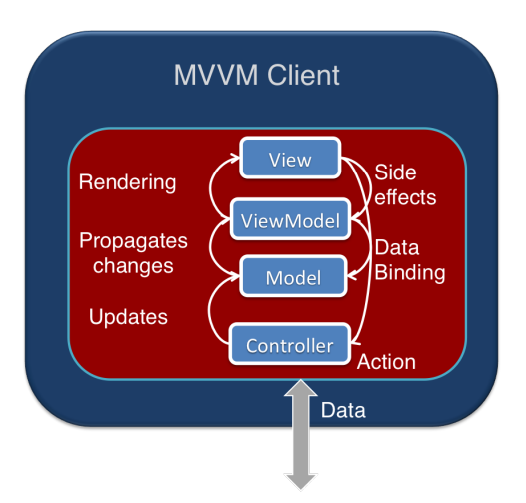
\includegraphics[width=0.5\linewidth]{figures/MVVM.png}
    \caption{Model View View-Model Model (\cite{zaris_-depth_nodate})}
    \label{fig:mvvm}
\end{figure}

\subsection{Angular}
\label{litrev:angular}
Angular has two separate versions, AngularJS (2010) and Angular2+ (2016); these are similarly both referred to as AngularJS; however, Angular2+ is the latest, maintained version based on Typescript, whereas AngularJS is built with JavaScript and is no longer actively maintained. Angular2+ is discussed within this review and will be referred to as Angular from now onwards.

Angular interacts with the DOM differently to React and Vue as Angular does not utilise the VDOM, instead handling only direct DOM manipulations (\cite{levlin_dom_2020}), but is still based on the MVC model \see{fig:mvc-model}. Angular interacts most similarly to JQuery out of all the modern frameworks. It implements create functions, such as \codeword{createCustomElement()}, which can be used to covert existing components into a class to be displayed on the DOM (\cite{levlin_dom_2020}). These classes contain decorators, which not only provide metadata but are also responsible for updating the component. Updates made to components via the decorator will update the existing DOM without the need to update a VDOM and compare it with the DOM (as done in React and Vue).

\section{Go (Programming Language)}
\label{litrev:golang}

Go, sometimes referred to as Golang, was developed by Google in 2007 and "arose through experience building large-scale distributed systems, working in a large codebase shared by thousands" (\cite{cox_go_2022}). Golang was built during a time when multi-core systems were becoming more and more common. Software Engineers at Google at the time found that the whole industry struggled to write efficient systems for multicore systems, and Go was their solution to the problem. Go has become increasingly popular over recent years \see{fig:gosograph}, primarily because the entire industry now faces those original issues highlighted by Google in 2007 when they were developing Go (\cite{cox_go_2022}).

Concurrency is one of Go's headline features. The language splits its concurrency model into two fundamental elements: Goroutines (lightweight threads) and Channels, which enable multiple Goroutines to communicate and synchronise execution (\cite{meyerson_go_2014}). Go follows the fork-join concurrency model; fork refers to how, at any point, it can split a child branch of execution which runs concurrently alongside the parent branch (\cite{cox-buday_concurrency_2017}). Once the child process has finished execution, it will rejoin the parent at the join \see{fig:forkjoin}.

\begin{figure}
    \centering
    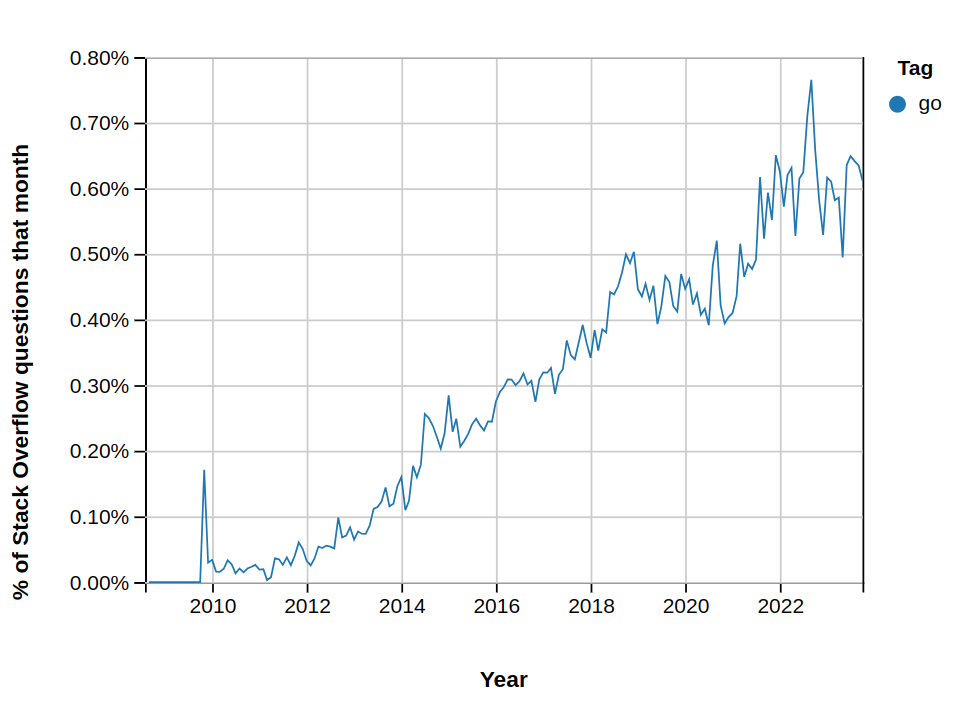
\includegraphics[width=0.8\linewidth]{figures/go-so-graph.png}
    \caption{Stack Overflow Trends Go (14/11/2023) (\cite{noauthor_stack_nodate-1})}
    \label{fig:gosograph}
\end{figure}

\begin{figure}
    \centering
    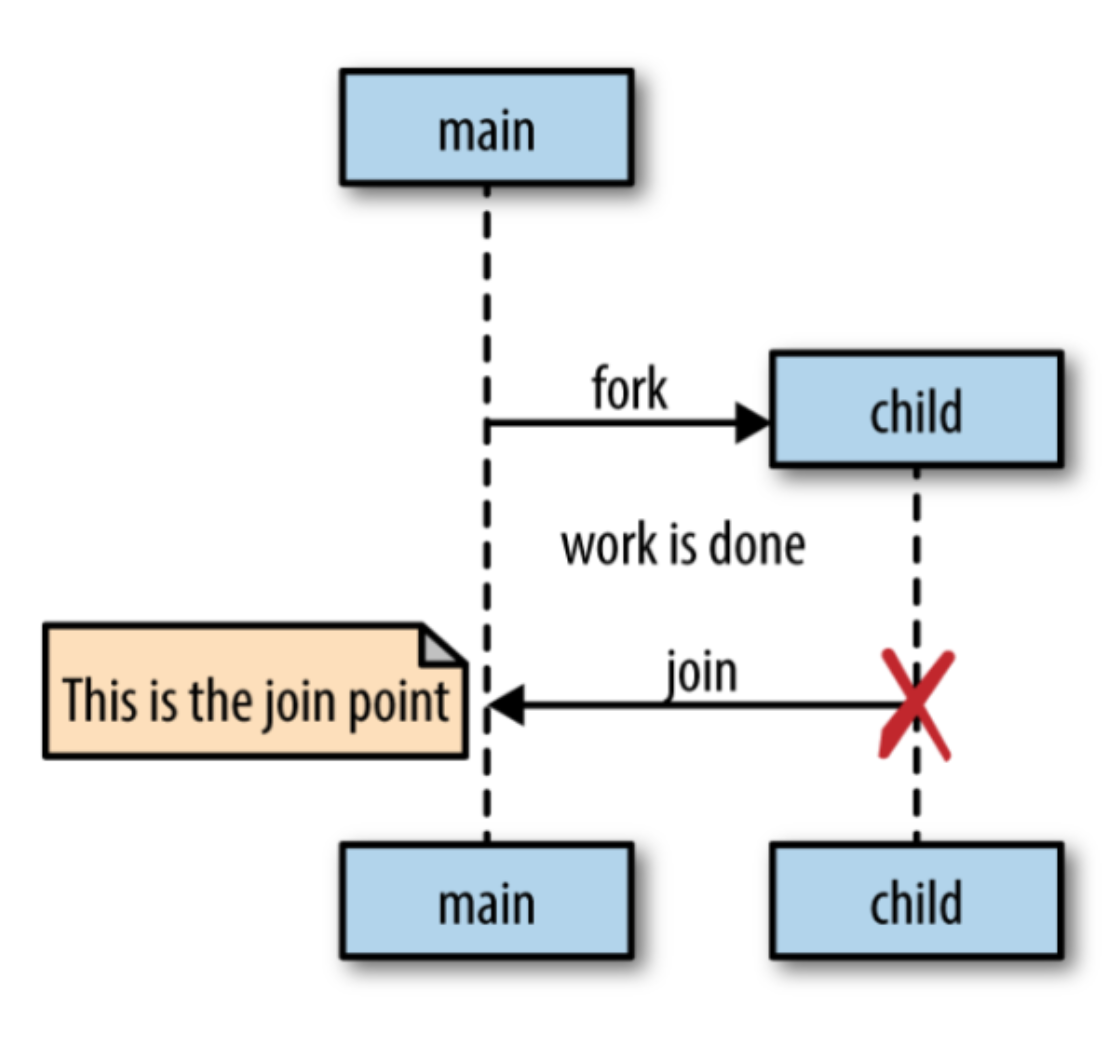
\includegraphics[width=0.5\linewidth]{figures/fork-join.png}
    \caption{Fork-Join Model (\cite{cox-buday_concurrency_2017})}
    \label{fig:forkjoin}
\end{figure}